\documentclass{article} % For LaTeX2e
\usepackage{iclr2018_conference,times}
\usepackage{hyperref}
\usepackage{url}
\usepackage{graphicx}
\usepackage{natbib}


\title{(tentative) Learning Neural Markers of Schizophrenia Disorder Using Recurrent Neural Networks}

% Authors must not appear in the submitted version. They should be hidden
% as long as the \iclrfinalcopy macro remains commented out below.
% Non-anonymous submissions will be rejected without review.

\author{Antiquus S.~Hippocampus, Natalia Cerebro \& Amelie P. Amygdale \thanks{ Use footnote for providing further information
about author (webpage, alternative address)---\emph{not} for acknowledging
funding agencies.  Funding acknowledgements go at the end of the paper.} \\
Department of Computer Science\\
Cranberry-Lemon University\\
Pittsburgh, PA 15213, USA \\
\texttt{\{hippo,brain,jen\}@cs.cranberry-lemon.edu} \\
\And
Ji Q. Ren \& Yevgeny LeNet \\
Department of Computational Neuroscience \\
University of the Witwatersrand \\
Joburg, South Africa \\
\texttt{\{robot,net\}@wits.ac.za} \\
\AND
Coauthor \\
Affiliation \\
Address \\
\texttt{email}
}

% The \author macro works with any number of authors. There are two commands
% used to separate the names and addresses of multiple authors: \And and \AND.
%
% Using \And between authors leaves it to \LaTeX{} to determine where to break
% the lines. Using \AND forces a linebreak at that point. So, if \LaTeX{}
% puts 3 of 4 authors names on the first line, and the last on the second
% line, try using \AND instead of \And before the third author name.

\newcommand{\fix}{\marginpar{FIX}}
\newcommand{\new}{\marginpar{NEW}}

%\iclrfinalcopy % Uncomment for camera-ready version, but NOT for submission.

\begin{document}


\maketitle

% Outline: 
% 1. Introduction: RNNs and CNNs being used for variety of recognition and diagnosis tasks. Problem with previous attempts
% to learn features from brain imaging data (fmri). High variability in brain responses across individuals.
% 2. Related Work: previous work on frmi, previous work to learn from videos, previous work to diagnose schizophrenia 
% 4. Methods
%   4.1 dataset
%   4.2 recurrent-convolutional neural nets for feature learning from fmri segments
% 5. Experiments: 
%   5.1 effectiveness of RNNs and R-CNNs to learn discriminative features from fmri
%	  5.2 generalizability of learned features across datasets
% 6. Discussion
% 7. Conclusion

\begin{abstract}
... Here we propose a new method based on recurrent-convolutional neural networks to automatically learn useful representations from short segments of fMRI recordings...
\end{abstract}

\section{Introduction}
*A key challenge in dealing with neuroimaging data comes from the inter- and intra-subject variability that any robust diagnosis system should be robust to. A prominent cause of these variabilities are due to small differences in the functional cortical mapping between individuals which calls for neural markers that are position and scale invariant.

INTRODUCTION
Diagnosis of psychiatric diseases can be a prolonged process. This is mainly due to lack of objective biological markers (such as the level of a metabolite in patient’s blood test) and similarity of symptoms among different diseases (e.g. depression phase of bipolar disorder and unipolar depression). Delayed and sometime inaccurate diagnosis results in belated less effective intervention. In addition, there is no objective biological marker for predicting treatment response in an individual. This oftentimes results in multiple changes in a patient’s prescription resulting in poor adherence given the medications side effects. Such inefficiency in diagnosis and treatment prognosis of psychiatric disorders is reflected in the global statistics [[burden of disease]] [[ as well as loca statistics]], with mental illness ranking first, before cancer and cardiac conditions, in terms of time lost to disability [WHO 2012 report] and costs \citep{Roehrig2016} [associated with the disease]. 

In recent years, machine learning techniques have shown success in identifying patients with mental or neurological disorders or predicting treatment response using brain imaging, especially structural and functional MRI (magnetic resonance imaging) data \citep{Gheiratmand2017, Orru2012, ?? Add more}. Almost all these studies extract features from imaging data and use the features in combination with standard classifiers, such as support vector machines (SVM) \citep{Orru2012, Wolfers2015} to discriminate between patients and controls or predict response to treatment [depression-new study]. (Less studies are available on the treatment response prediction, mainly due to lack of treatment response data, compared to diagnostics data) (Some typical imaging features extracted from fMRI or MRI include functional connectivity [], ALFF (amplitude of low-frequency fluctuations) [] for fMRI data, and voxel-based morphometry [], or gray matter thickness/volume [] for structural MRI. Such features may be extracted voxel-wise (where every voxel is a brain tissue of size ~1-33 mm3) or region-wise from predefined brain regions (such as thalamus, postcentral gyrus, etc.)

With deep learning techniques gaining outstanding performance in various fields including image classification [Refs], speech recognition [Refs], and video classification [Refs], among others, the approach is being recruited and explored in clinical applications, including those involving medical imaging data \citep{Shen2017, Litjens2017, Gulshan2016} [need comments on CNN? Re its vast use]. In addition to their potential to surpass the performance of other standard machine learning methods, deep learning methods are attractive because they can be directly applied to the data, skipping the need to extract hand-engineered features from the data – a step that is necessary in almost all other machine learning approaches [check statement correctness]. Deep Neural Networks might [or has the potential to] learn representations from brain images that might reveal useful information about abnormalities associated with the disease [check statement correctness]. 

Various deep learning methods have been employed in analysis of imaging data for various psychiatric and neurological disorders, including but not limited to Alzheimer’s disease (AD), ADHD, and Psychosis (see \citep{Vieira2017}). These methods include multi-layer perceptron (MLP), autoencoders (AE), deep belief networks, and convolutional neural networks citep[see][]{Vieira2017}[][for a review]. Most of these studies use structural MRI for predictions in neurological disorders, and much fewer studies use fMRI, which has been shown to be particularly relevant in predictive analysis of psychotic disorders (such as schizophrenia) (e.g. \citep{Damaraju2014, Calhoun2009}). fMRI data measures blood oxygen-level dependent signal (BOLD) at every brain voxel by taking a scan of the whole brain every 1-3 s. It can be thought of as a movie of the brain activity (reflected in BOLD signal – although the relationship between BOLD and neural activity is still under scrutiny [Ref-Amir Shmuel]), either in response to a task (e.g. a motor, sensory, or cognitive task) or simply at rest. 	\citet{Plis14} did this xxx …. \citet{Sarraf2016}[[bio]arxive][include??] did this xxx ..... \citet{Kim2016} used functional connectivity features with xxx ...  \citet{Suk2016} [[discuss here??]

Here, our goal was to exploit both spatial and temporal information in the fMRI movie for identifying patients with schizophrenia. As mentioned earlier, most previous fMRI/machine learning studies, including some deep learning ones \citep{Kim2016}, use hand-crafted features, in particular functional connectivity \citep{Gheiratmand2017}, which collapses the time dimension (of the BOLD signal) into one single number (i.e. the correlation coefficient between a pair of time-series), and does not keep track of the relationships between spatial locations (e.g. voxel or brain regions). Here, we propose using a recurrent convolutional neural network to exploit both spatial and temporal information in fMRI data. The model involves a 3-D CNN network followed by an LSTM network. The CNN will extract spatial features, which are then fed to the LSTM model that uses the dependencies between time points at every spatial location to generate an output {patient, control}. To our knowledge, this is the first work to apply a recurrent CNN to fMRI data for identifying patients with a mental disorder (here schizophrenia). We expanded the work by \citet{Bashivan2015}, who successfully applied a recurrent CNN (with 2D convolutions) to EEG data in a mental load classification task, to fMRI data (3D convolutions). [[video classification idea]] We used fMRI data in response to an auditory oddball task and a working memory task from patients diagnosed with schizophrenia and healthy controls from FBIRN dataset [Ref]. The task is to predict a label {patient, control} based on the preprocessed fMRI BOLD signal per voxel. [[In the next sections, we will first describe ...]]

   
[FBIRn data -- previously used with standard ML techniques and FC features [npj schz]]


\section{Related Work}



\section{Methods}

\subsection{Dataset}
One scan was captured every 2 seconds. Each session (??) consists of a single fMRI scanning session which lasted for almost 5 minutes (??). Data from each session was split to windows of 32 or 128 seconds which formed the samples used for training, evaluation, and test.  

\subsection{Recurrent-Convolutional Neural Networks}
We compared accuracy of recurrent neural networks (LSTM model) and recurrent-convolutional nerual networks (R-CNN) with baseline classifiers to learn discriminative features for the problem of distinguishing normal and schizophrenic individuals. We tried several different architectures consisting of LSTMs as well as R-CNNs. The input data was structured as a 3-dimensional tensor (3D brain scans). 

\textbf{Baseline Classifier}: We used a $L_1$-regularized logistic regression model and Support Vector Classifier (SVC) applied on voxel activations as the baseline models to compare against. Both of these models were trained on voxel values on all time-frames (did we do this??). 

\textbf{LSTM model}: All voxel values are reshaped into a vector and fed directly into a two-layer forward LSTM model. LSTMs are known for their ability in learning long-term dependencies between inputs. In this model the spatial relationship between voxels are ignored and LSTM learns the temporal relationship between activations in different voxels. 

\textbf{Conv-LSTM model}: 3-D activations for each time frame were fed into a 3D CNN. We used 3-dimensional convolutions followed by max-pooling to extract position and scale independent features that would generalize across individuals. Identical networks were used to process each time-frame with shared weights between them. Outputs of each CNN were then reshaped into a vector that was fed as input to the LSTM network at each time step. Figure-\ref{fig1} shows an overview of the recurrent-convolutional network used here. CNN part learns 3-D features that are invariant to translation and scaling and reduces the dimension of the input space before feeding it into LSTM. 

A batch size of 64 was used for all models. Larger convolutional models were trained synchronously on 16 GPUs. In both cases we experimented with varying number of time-frames included in each sample (i.e. 16 and 64).

\subsection{Training Details}
\label{training_details}
We used Adam optimizer with default parameter settings ($\beta_1=0.9, \beta_2=0.999, \epsilon=10^{-8}$). We included dropout in the input and outputs of the LSTM cells \citep{Zaremba2014} which contained most of the tunable parameters in our models. 

10-fold cross-validation was used to evaluate the performance for each proposed model. $l_2$ regularizer was used on all convolutional and fully connected weights. 
3D-convolutions of size $3\times3\times3$ with stride 1 were used. Each block of convolutions were followed by a maxpool layer of size 2 and stride 2. Feature map size was dividing by 2 after each maxpool layer. Size of the input to the network was $(53\times64\times37)$.

A different subset of subjects were assigned to the test set for each fold and data from the rest of the subjects were used for training and validation (without overlap between train and validation sets). For training, samples within each batch were generated by randomly selecting time windows from different subjects. All possible time windows of size $T$ from all subjects were used for training, validation and test. For each fold training was done for 10 folds. We used the validation set to for early stopping of training. After each training epoch, performance on the validation set was computed. Training was performed for 10 epochs and test performance was computed for the network state with highest validation score. 



\begin{figure}[t]
\begin{center}
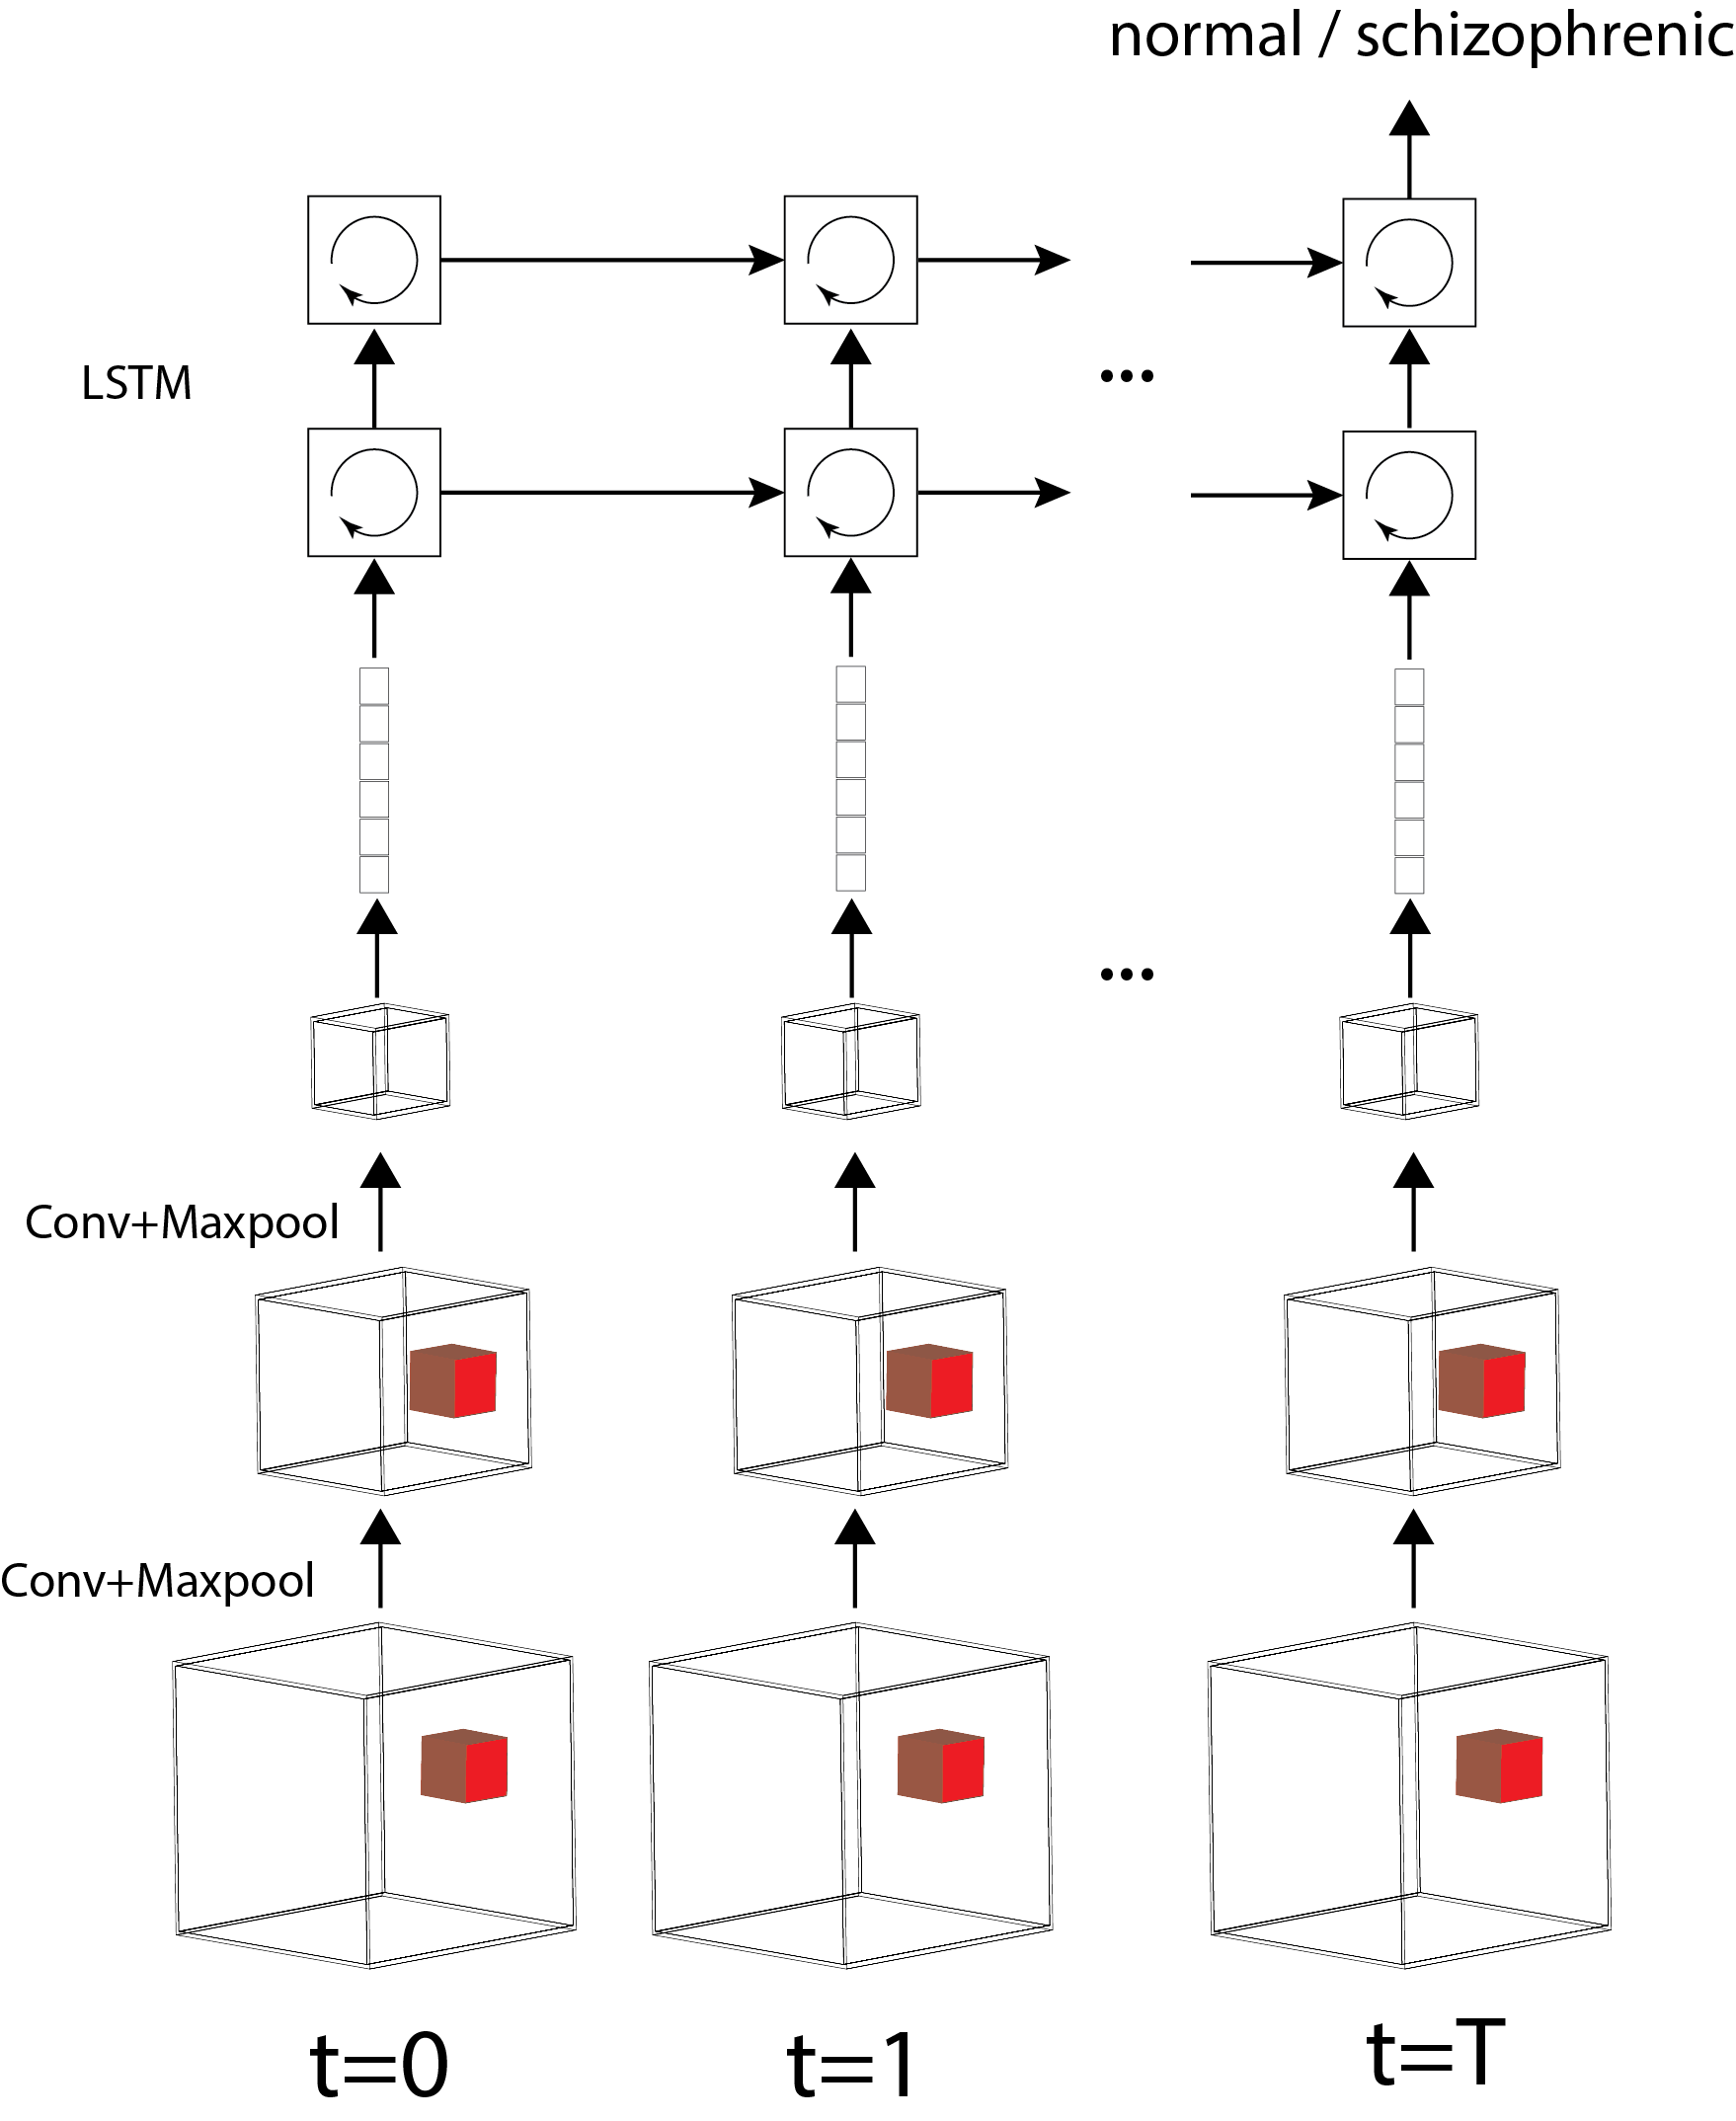
\includegraphics[width=3in]{figures/overview.png}
\end{center}
\caption{Overview of the method used.}
\label{fig1}
\end{figure}

\subsection{Data Preprocessing}
Data preprocessing was done in three steps. (i) For each subject-run the average voxel activation was subtracted; (ii) each subject-run was 

\subsubsection*{Acknowledgments}

Use unnumbered third level headings for the acknowledgments. All
acknowledgments, including those to funding agencies, go at the end of the paper.

\bibliography{iclr2018_conference}
\bibliographystyle{iclr2018_conference}

\end{document}
